\documentclass[subsection=false, compress]{beamer}
\setbeamertemplate{footline}[frame number] % numerar slides
\setbeamertemplate{navigation symbols}{} % retirar barra de navega��o
% \setbeamertemplate{background}{\tikz[overlay,remember picture]\node[opacity=1]at (current page.center){\includegraphics[width=\paperwidth, height=\paperheight]{Figures/water-mark}};}

\mode<presentation>
\usetheme{Singapore}
%\usefonttheme{structurebold}
%\usebeamercolor[fg]{section in sidebar}

\ifdefined\hyperref

\usepackage[brazil]{babel}
\usepackage[latin1]{inputenc}
\usepackage{subfig}
\usepackage{graphicx}
%\usepackage{subcaption}
\usepackage{pgfpages}
\usepackage{ifpdf}
\usepackage{multimedia}
\usepackage{color}
\usepackage{url}
\usepackage{hyperref}
\usepackage{lastpage}
\usepackage{graphicx}
\usepackage{listings}
\usepackage{listing}
\usepackage{nameref}
\usepackage{array}
\usepackage{marvosym}
\usepackage{multicol}
\usepackage{pifont}
\usepackage{marvosym}
\usepackage{cancel}
%\usepackage{enumitem}
%\usepackage{minted}
%\usepackage{subfigure}
%\usepackage{xmpmulti}
%\usepackage{animate}
\usepackage[export]{adjustbox}
\usepackage{changepage}
\usepackage{lipsum}
\usepackage{tikz}
\usepackage{kantlipsum}
\usepackage{booktabs}

\definecolor{erick}{HTML}{7CFC00}
\definecolor{suzane}{HTML}{006400}


\lstset{%
	linewidth=\textwidth,%framed box is the text size
	xleftmargin=.10in,
	xrightmargin=.10in,
	frame=trbl,
	columns=flexible,
	captionpos=t,
	upquote=false,
	basicstyle=\footnotesize\ttfamily,
	firstnumber=1,%
	numberfirstline=false,%
	numbers=left,%
	numberstyle=\tiny,%
	stepnumber=1,%
	numbersep=5pt,%
	backgroundcolor=\color{blue!15},%
	tabsize=4,%
	keywordstyle=\color{green!65!black},%
	commentstyle=\color{blue},%
	stringstyle=\color{magenta},%
	breaklines=true,%
	emph={label},%
	abovecaptionskip=10pt,%
	belowcaptionskip={\abovecaptionskip},%
	showstringspaces=false,
	escapeinside=@@,%
	literate={�}{{\^{E}}}1
}%
\usepackage{textpos} % package for the positioning

% position the logo
% \addtobeamertemplate{frametitle}{}{%
% 	\begin{textblock*}{100mm}(\textwidth,6.70cm)
		% 
\includegraphics[height=1.00cm,width=1.00cm,keepaspectratio]{Figures/logo_ufpa}
	% \end{textblock*}
	%\begin{textblock*}{100mm}(-0.80cm,-0.25cm)
	%\begin{textblock*}{100mm}(-0.80cm,6.90cm)
	%	\includegraphics[height=1.00cm,width=1.00cm,keepaspectratio]{Figures/ihc}
	%\end{textblock*}
% }

%%\pgfdeclareimage[width=0.85cm, height=1.10cm]{ufpa}{Figures/logo_ufpa}
%\pgfdeclareimage[width=1.60cm, height=1.00cm]{ufpa}{Figures/foot_img}
%\logo{\pgfuseimage{ufpa}}

\hypersetup{
    pdftitle={Uso de Redes Neurais Profundas e Recorrentes para Reconhecimento de Fala em Portugu�s Brasileiro}
	pdfauthor={Jo�o Victor da Silva Dias Canavarro}
}
\fi

\makeatletter
\newcommand*{\currentname}{\@currentlabelname}
\makeatother

% http://tex.stackexchange.com/questions/50286/beamer-singapore-theme-follow-up-line-above-footline-and-hide-footline-for-si
%\setbeamercolor{footlinerule}{use=structure,bg=structure.fg!25!bg,green}
\setbeamertemplate{footline}
{%
	\begin{beamercolorbox}[wd=\paperwidth,ht=0.5ex,dp=0ex,center]{footlinerule}
	\end{beamercolorbox}%
	\begin{beamercolorbox}[wd=\paperwidth,ht=0.6ex,dp=0ex,center]{empty}
	\end{beamercolorbox}%
	\leavevmode%
	\hbox{%

	\begin{beamercolorbox}[wd=.20\paperwidth,ht=2.25ex,dp=2ex,center]{author in head/foot}%
		\usebeamerfont{author in head/foot}%
		\insertshortauthor\hspace{1em}%(FCT/\insertshortinstitute)
	\end{beamercolorbox}%

	\begin{beamercolorbox}[wd=.45\paperwidth,ht=2.25ex,dp=2ex,right]{title in head/foot}%
		\usebeamerfont{title in head/foot}
		\insertshorttitle
	\end{beamercolorbox}%

	\begin{beamercolorbox}[wd=.20\paperwidth,ht=2.25ex,dp=2ex,right]{author in head/foot}%
		\usebeamerfont{author in head/foot}%
		\textbf{\textcolor{black}{\currentname}}
	\end{beamercolorbox}%

	\begin{beamercolorbox}[wd=.10\paperwidth,ht=2.25ex,dp=2ex,right]{date in head/foot}%
		\textbf{\textcolor{black}{\insertframenumber{} de \inserttotalframenumber\hspace*{1ex}}}
	\end{beamercolorbox}}%
	\vskip0pt%
}%

%\title[Universal Remote Control System with AGR]
%{\Large A Proposal of a Universal Remote Control System Based on Head Movements}
%
%\author[Cassio T. Batista]
%{\large
%\textbf{Cassio Trindade Batista}\\
%Erick Modesto Campos\\
%Nelson Cruz Sampaio Neto
%\vspace{.2cm}
%}

%\institute[UFPA]{
%\small
%Universidade Federal do Par�\\[1pt]
%%Programa de P�s-Gradua��o em Ci�ncia da Computa��o\\[1pt]
%Laborat�rio de Visualiza��o, Intera��o e Sistemas Inteligentes\\[1pt]
%Bel�m -- Par� -- Brazil\\[1pt]
%\begin{figure}
%	
\includegraphics[width=.13\textwidth]{Figures/logo_ufpa}
%\end{figure}
%\vspace{-0.40cm}
%}
%\date{
%\small
%25 de outubro de 2017
%}
% \title[Acionador Externo de Baixo Custo Baseado em Sopro]
\title[Uso de DNNs para Reconhecimento de Fala em PT\_BR]
% {\Large Uma Proposta de Acionador Externo de Baixo Custo Baseado em Sopro}
% {\Large Uma Proposta de Controle Alternativo do Mouse Centrado na Cabe�a do Usu�rio}
{\Large Uso de Redes Neurais Profundas e Recorrentes Para Reconhecimento de Fala
em Portugu�s Brasileiro -- Parte II}
\author[ Jo�o V. Canavarro ]
{\large \textbf{Jo�o Victor da Silva Dias Canavarro}\vspace{.2cm}}

\institute[UFPa]{
\small
Instituto de Ci�ncias Exatas e Naturais\\[1pt]
Faculdade de Computa��o\\[1pt]
Laborat�rio de Visualiza��o, Intera��o e Sistemas Inteligentes\\[1pt]
% Aluno: Jo�o Victor da Silva Dias Canavarro
Orientador: Prof. Dr. Nelson Cruz Sampaio Neto \\
\begin{figure}

\includegraphics[width=.12\textwidth]{Figures/logo_ufpa}
\end{figure}
\vspace{-.35cm}
}
\date{\small{25 de Agosto de 2021}}

\begin{document}
% ------------------------------------------------------------------------------
\begin{frame}[plain]
	\titlepage
\end{frame}

% ------------------------------------------------------------------------------
% \begin{frame}{Agenda}
% \begin{enumerate}
% 	\item Introdu��o
% 	\bigskip

% 	\item Prot�tipo
% 	\bigskip

% 	\item Testes e Resultados
% 	\bigskip

% 	\item Conclus�es e Trabalhos Futuros
% \end{enumerate}
% \end{frame}

% ------------------------------------------------------------------------------
%%%%%%%%%%%%%%%%%%%%%%%%%%%%%%%%%%%%%%%%%
%%% begin of body
%%%%%%%%%%%%%%%%%%%%%%%%%%%%%%%%%%%%%%%%

\section{Introdu��o}
%%%%%%%%%%%%%%%%%%%%%%%%%%%%%%%%
\subsection{Introdu��o}
% ----------------------------------------------------------------------------
% \begin{frame}{Introdu��o}
% \begin{itemize}
% 	\item Intera��es convencionais:
% 	\begin{itemize}
% 		\normalsize
% 		\smallskip
%         \item[--] Teclado, \textit{mouse}, \textit{touchscreen}, \textit{joystick}, controle remoto, etc.
% 	\end{itemize}
% 	\smallskip
% \end{itemize}
% % \vspace{-0.5cm}
% \begin{figure}
% 	\includegraphics[width=0.3\textwidth]{Figures/mouse1} \quad
% 	\includegraphics[width=0.2\textwidth]{Figures/toque}
% \end{figure}

% \begin{itemize}
% 	\item Intera��es n�o convencionais:
% 	\begin{itemize}
% 		\normalsize
% 		\smallskip
%     \item Acionadores externos, controle por voz, etc.
% 	\end{itemize}
% \end{itemize}
% \begin{figure}
% 	% \includegraphics[width=0.2\textwidth]{Figures/talk} \quad
% 	% \includegraphics[width=0.4\textwidth]{Figures/ta} \quad
% 	\includegraphics[width=0.2\textwidth]{Figures/icon_asr}
% \end{figure}
% \end{frame}

% \begin{itemize}
%     \item Aplica��es:
%     \begin{itemize}
%         \item Tecnologias assistivas, \textit{eye-trackers}, estudos em lingu�stica, s�ntese de voz
%     \end{itemize}
% \end{itemize}

% ----------------------------------------------------------------------------
%\begin{frame}{Por que utilizar Acionadores?}
%\begin{itemize}
%	\item Acessibilida
%	\smallskip
%	\item Melhoram a intera��o humano-computador (IHC)
%	\smallskip
%	\item Comodidade e conforto
%\end{itemize}
%\begin{figure}
%	\includegraphics[width=0.48\textwidth]{Figures/jarvis02}
%\end{figure}
%\end{frame}

%%%%%%%%%%%%%%%%%%%%%%%%%%%%%%%%
% \subsection{Motiva��o}
% % ----------------------------------------------------------------------------
% \begin{frame}{Motiva��o}
% \begin{itemize}
% 	\item \textbf{Acessibilidade}: TA para PCD \medskip
% 	\item Tecnologia Assistiva voltada �s pessoas com defici�ncia
% \end{itemize}
% \begin{figure}
% 	\includegraphics[width=0.80\textwidth]{Figures/access_1}
% \end{figure}
% \end{frame}

% ----------------------------------------------------------------------------
%\begin{frame}{Estat�sticas da Popula��o com Defici�ncia}
%\begin{itemize}
%	\item Mundialmente: 15\% da popula��o $\approx$ 1 bilh�o de
%	pessoas~\textcolor{gray}{\small[OMS, 2015]}
%	\medskip
%	\item No Brasil: 23,9\% dos brasileiros $\approx$ 46 milh�es de
%	pessoas~\textcolor{gray}{\small[IBGE, 2010]}
%\end{itemize}
%\begin{table}
%\centering
%\caption{Perfil da popula��o brasileira com defici�ncia}
%\begin{tabular}{lcr}
%	\hline
%	\hline
%	{\bf Defici�ncia} & {\bf N�mero de Pessoas} & {\bf Porcentagem} \\
%	\hline
%	{Visual}          & {35.774.392}            & {18,754}     \% \\
%	{\bf Motora}      & {\bf 13.265.599}        & {\bf 6,95}   \% \\
%	{Auditiva}        & 9.717.318               & 5,094        \% \\
%	{Cognitiva}       & 2.611.536               & 1,369        \% \\
%	\hline
%	\hline
%\end{tabular}
%\end{table}
%\end{frame}

%\begin{frame}{Problemas}

%    \begin{itemize}
%    \item Intera��es Convencionais for�am o uso das m�os
%    \item Falta de acessibilidade para PCD
%    \item Pre�o dos dispositivos existentes
%    \end{itemize}

%\end{frame}

%\begin{frame}{Dispositivos Dispon�veis - Detector de Pisque}
%	\includegraphics[width=\textwidth]{Figures/blink_switch}
%\end{frame}

%\begin{frame}{Dispositivos Dispon�veis - Detector de Sopro}
%	\includegraphics[width=\textwidth]{Figures/puff}
%\end{frame}

%\begin{frame}{Dispositivos Dispon�veis - {Mouse Tracker} com Girosc�pio}
%    \begin{itemize}
%        \item \url{zyteq.com}
%    \end{itemize}
%	\includegraphics[width=\textwidth]{Figures/zono}
%	\includegraphics[width=\textwidth]{Figures/price}
%\end{frame}

%\subsection{Proposta}
%% ----------------------------------------------------------------------------
%\begin{frame}{Proposta do Trabalho}
%\begin{itemize}
%	\item Controlador de mouse baseado na cabe�a do usu�rio
%	\begin{itemize}
%		\normalsize
%		\medskip
%		\item[--] M�todo alternativo de clique
%		\item[--] Multiplataforma
%		% \begin{itemize}
%		% 	\normalsize
%		% 	\item[$\hookrightarrow$] Linux
%		% \end{itemize}
%		%\smallskip
%		\item[--] Livre: \textit{open-source} e \textit{open-hardware}
%		\item[--] De baixo custo
%		\smallskip
%		\item[--] Com foco em acessibilidade
%		\begin{itemize}
%			\smallskip
%			\normalsize
%			\item[$\hookrightarrow$] PCD motora dos membros superiores
%			(MMSS)
%            \item[$\hookrightarrow$] Movimento cognitivo e da cabe�a preservado

%		\end{itemize}
%	\end{itemize}
%\end{itemize}
%\end{frame}




%\subsection{Justificativa}
%% ----------------------------------------------------------------------------
%\begin{frame}{Justificativa}
%\begin{itemize}
%\item Por que utilizar o sopro e movimenta��o da cabe�a do usu�rio como m�todo de controle?
%\end{itemize}
%\begin{itemize}
%	\item No meio acad�mico:
%	\smallskip
%	\begin{itemize}
%		\normalsize
%		\item Dificuldade em encontrar trabalhos que utilizam
%acionadores como m�todo alternativo de clique e movimenta��o do mouse
%		\smallskip
%		\item Apenas um trabalho de acionador externo baseado em
%sopro~\textcolor{gray}{\small[B. Aigner, 2016]}
%		\smallskip
%		\item  Poucos detalhes do desenvolvimento de
%		acionadores externos
%		\smallskip
%	\end{itemize}
%\end{itemize}

%\end{frame}


%\begin{frame}{Justificativa}
%%
%\begin{itemize}
%	\item No mercado:
%	\smallskip
%%\begin{minipage}{0.65\textwidth}
%\begin{itemize}
%	\item[]
%\begin{itemize}
%	\normalsize
%	\item  Comunica��o direta atrav�s da interface de �udio para realizar o clique
%	\smallskip
%	\item  Acionadores externos de alto custo e propriet�rios
%\end{itemize}
%\end{itemize}
%\end{itemize}
%%\end{minipage}
%\begin{figure}
%	\centering
%	\includegraphics[width=0.3\textwidth]{Figures/ts1}\\
%	\includegraphics[width=0.3\textwidth]{Figures/at_switch_wireless} \quad
%	\includegraphics[width=0.3\textwidth]{Figures/at1}
%\end{figure}
%\end{frame}
%%% EOF %%%


\section{Objetivo}
%%%%%%%%%%%%%%%%%%%%%%%%%%%%%%%%
\subsection{Objetivo}
% ----------------------------------------------------------------------------
\begin{frame}{Reconhecimento de Voz}

\begin{figure}
	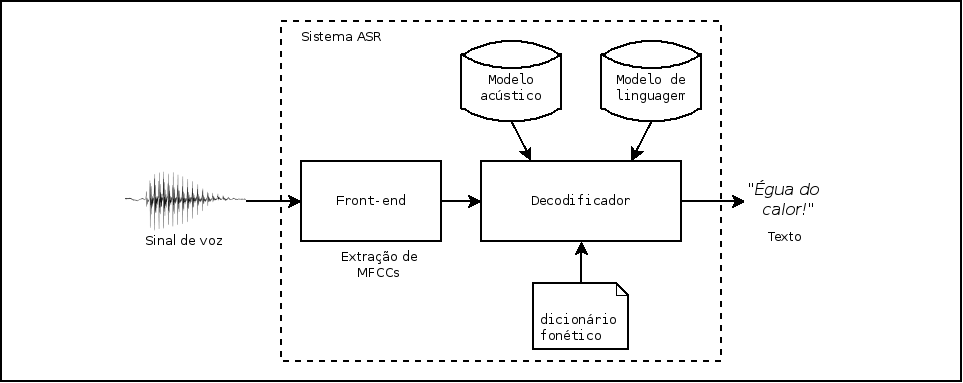
\includegraphics[width=0.9\textwidth]{Figures/asr}
    \caption{Esquema tradicional de um sistema autom\'atico de reconhecimento de voz}
\end{figure}

\begin{itemize}
    \item Aplica\c c\~oes:
    \begin{itemize}
        \smallskip
		\item Tecnologias assistivas, \textit{eye-trackers}, lingu\'istica (\textbf{alinhamento fon\'etico}), s\'intese de voz
    \end{itemize}
\end{itemize}
\end{frame}


\begin{frame}
\frametitle{Alinhamento Fon\'etico For\c cado}
	\begin{itemize}
		\item Automatiza\c c\~ao  da transcri\c c\~ao e alinhamento de fala gravada
		\item Estudo e pesquisa de linguistas
		\item Desenvolvimento de ferramentas mais robustas de reconhecimento e sintese de fala
	\end{itemize}
	\begin{figure}
	\begin{center}
		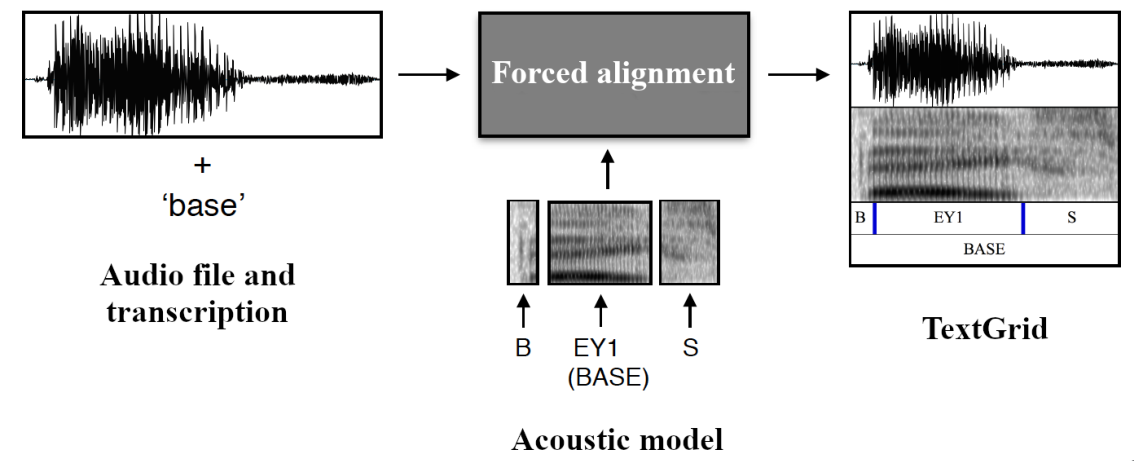
\includegraphics[width=0.8\textwidth]{Figures/align}
	\end{center}
	\end{figure}


\end{frame}


\begin{frame}{Ferramentas}
    \begin{itemize}
        \item Kaldi: um pacote \textit{open-source} de reconhecimento de voz
			\begin{itemize}
				\item Possui suporte para ambas HMM-GMMs (mistura de gaussianas) e HMM-DNNS (redes neurais profundas)
				\item Suporte para PT-BR
			\end{itemize}
		\begin{figure}
		\begin{center}
			
\includegraphics[width=0.4\textwidth]{Figures/kaldi}
		\end{center}
		\end{figure}

        \item Praat: \textit{software} utilizado por linguistas na  an\'alise da fala


        \item UFPAlign: alinhador fon\'etico autom\'atico baseado no HTK disponilizado pelo grupo Fala Brasil
    \end{itemize}
\end{frame}


\begin{frame}{Objetivo}
\begin{itemize}
    % \item Desenvolver um sistema de reconhecimento de voz para PT\_BR utilizando o pacote Kaldi para treinamento dos AMs e LMs
	\item Desenvolver um alinhador fon\'etico para PT\_BR baseado nos modelos
        ac\'usticos explorados no projeto anterior utilizando o Kaldi
	\begin{itemize}
		\item \textit{Plug-in} para o Praat
		\item Modelos ac\'usticos (AMs) treinados utilizando DNNs e HMM-GMMs
	\end{itemize}
	% \item Coletar dados para realizar \textit{LM rescoring}: 4-5 milh\~oes de frases
	\item Substituir o HTK na antiga ferramenta utilizada pelo grupo Fala
        Brasil com o objetivo de melhorar os resultados obtidos
    \item Disponibilizar recursos \`a comunidade cient\'ifica: grupo Fala Brasil
\end{itemize}

\begin{figure}
\begin{center}
	
\includegraphics[width=0.3\textwidth]{Figures/falabrasil}
\end{center}
\end{figure}

\end{frame}

%
\section{Metodologia e Testes}
\subsection{Metodologia}

% \begin{frame}
%     \frametitle{Metodologia}
%     \framesubtitle{Treinamento dos AMs}
%     \begin{center}
%         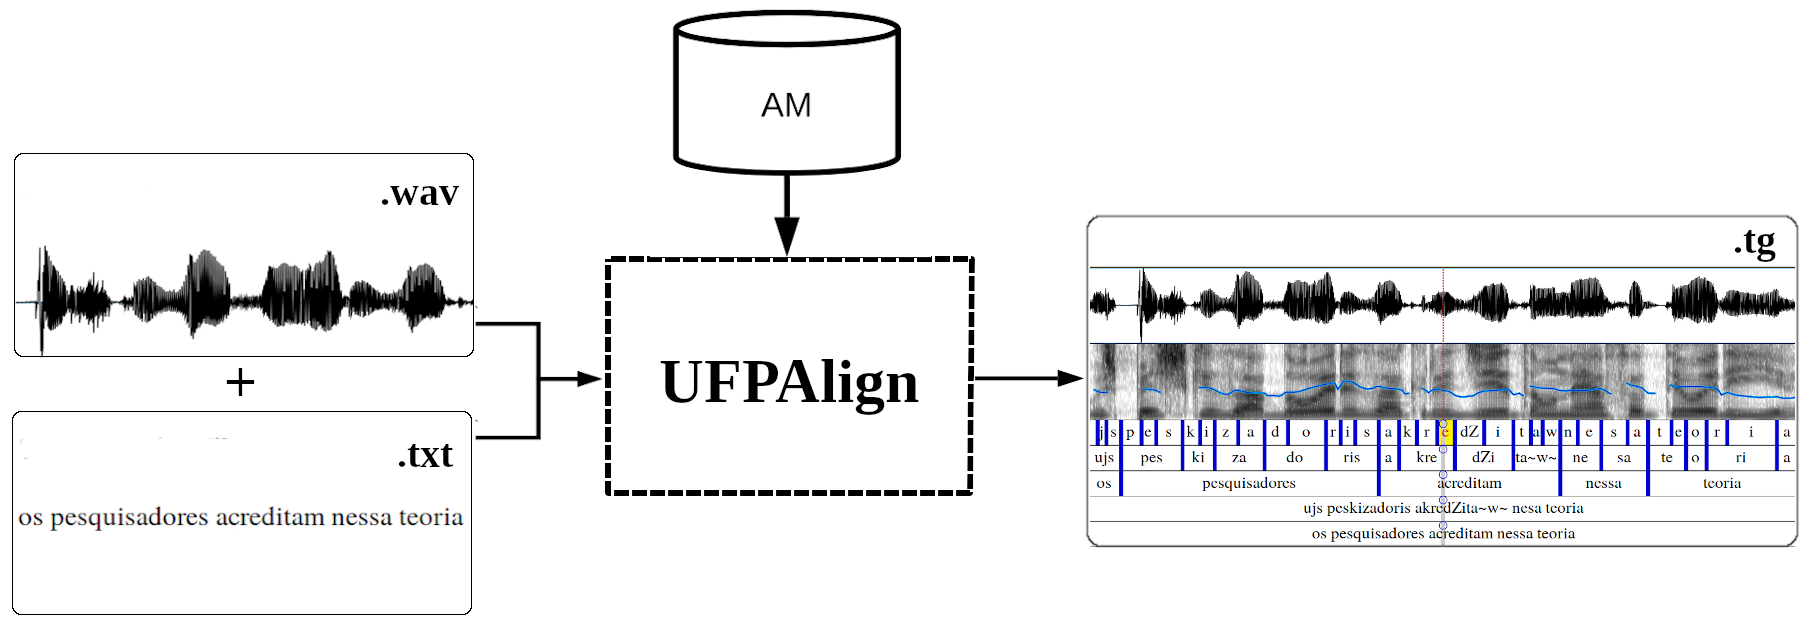
\includegraphics[width=1\textwidth]{Figures/ufpalign_geral}
%     \end{center}
% \end{frame}

\begin{frame}
    \frametitle{Metodologia}
    \framesubtitle{Base de \'Audio Transcrita}
    \begin{center}
        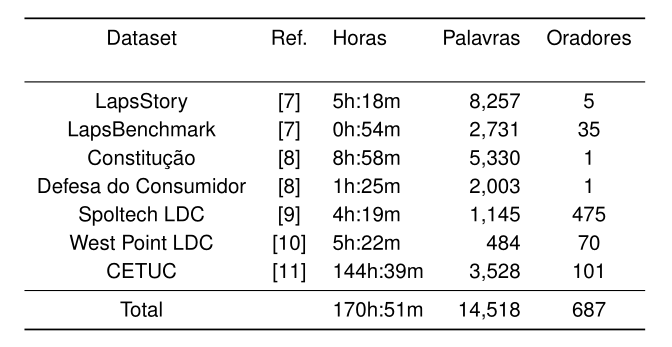
\includegraphics[width=0.8\textwidth]{Figures/db}
    \end{center}
\end{frame}

\begin{frame}
    \frametitle{Metodologia}
    \framesubtitle{Treinamento dos AMs}
    \begin{center}
        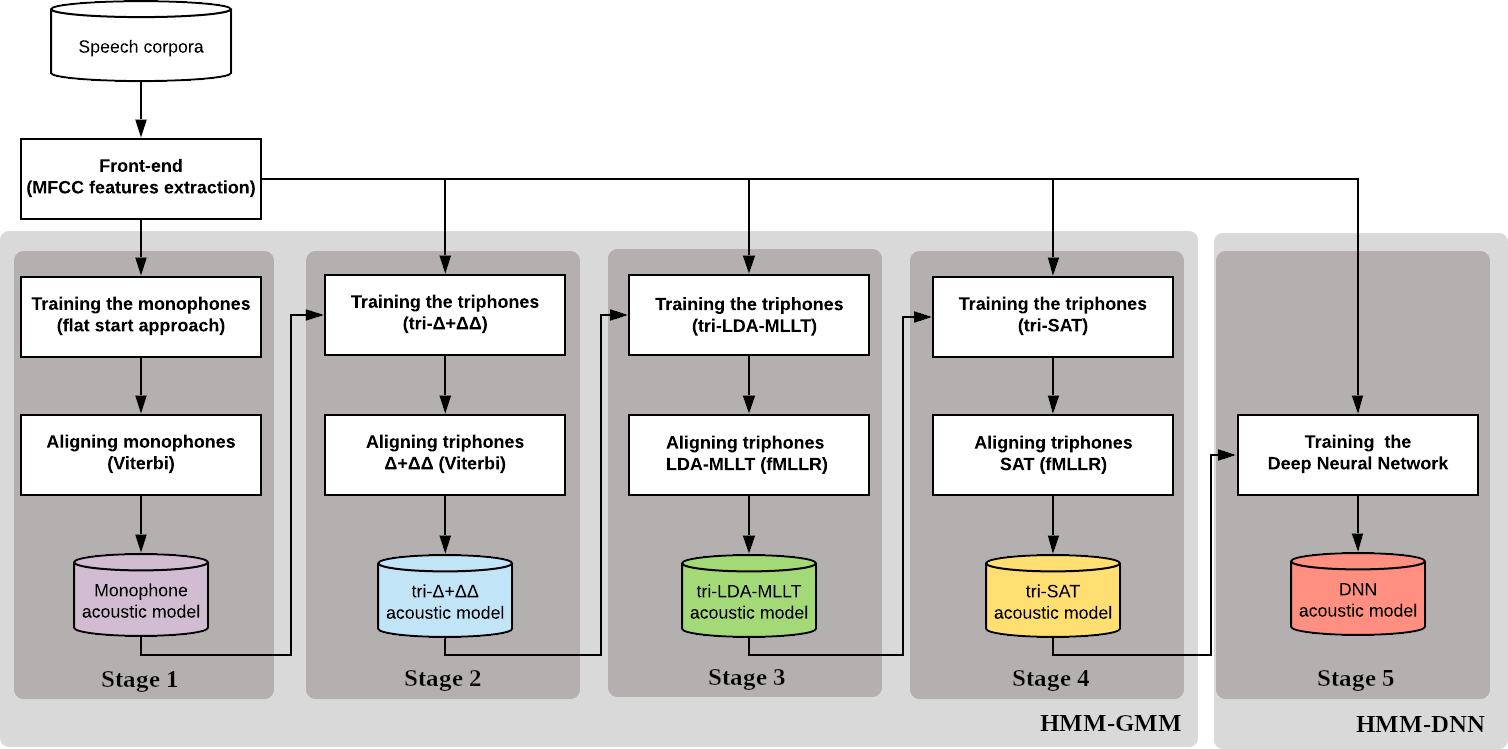
\includegraphics[width=1\textwidth]{Figures/kaldi_pipeline}
    \end{center}
\end{frame}

\begin{frame}
    \frametitle{Testes}
    \begin{itemize}
        \item \textit{Dataset} de Avalia\c c\~ao
        \begin{itemize}
            \item \'Audios de enunciados separados entre um locutor masculino (M) e um feminino
                (F)
            \item Arquivos \textit{TextGrid} de cada \'audio alinhados
                manualmente por um foneticista
        \end{itemize}
        \item Caracter\'istica comparada: limite fon\'etico
        \begin{itemize}
            \item Diferen\c ca entre o tempo final da ocorr\^encia do fonema em ambos alinhamentos, pelo alinhador e alinhado manualmente
        \end{itemize}
    \end{itemize}
\end{frame}

%
\section{Resultados e Conclus�es}
\subsection{Resultados}
\begin{frame}
    \frametitle{Resultados}
\begin{table}[!h]
\centering
\tiny
% \setlength{\tabcolsep}{5pt}
\renewcommand{\arraystretch}{1.1}
% \def\arraystretch{1.15}
\begin{tabular}{lccccccc}
\cmidrule{5-8}
                                &              &              &              & \multicolumn{4}{c}{Toler�ncia}    \\
                                \toprule
Modelo             & $\mu$      & mediana & $\sigma$                           & \textit{\textless 10ms} & \textit{\textless 25ms} & \textit{\textless 50ms} & \textit{\textless 100ms} \\ \hline
UFPAlign (HTK) - M  & {26.86} & \text{17.00} &      \multicolumn{1}{c|}{32.61} &        {30.73\%} &        {62.45\%} &        {86.55\%} &        {~96.42\%}  \\
    EasyAlign - M   & \text{24.35} & \text{17.00} & \multicolumn{1}{c|}{30.70} &   \text{31.53\%} &   \text{67.51\%} &   \text{89.69\%} &   \text{~96.95\%}  \\
Kaldi Mono - M     & 15.252 & 11.000  & \multicolumn{1}{c|}{15.704} & 43.51\%                 & 83.42\%                 & 96.29\%                 & 99.42\%                  \\
Kaldi tri-$\Delta$ - M & \textbf{14.158} & \textbf{10.000}  & \multicolumn{1}{c|}{14.057} & \textbf{46.28\%}                 & \textbf{\textbf{85.55\%}}                 & 97.13\%                 & 99.74\%                  \\
Kaldi tri-LDA - M  & 14.657 & 11.000  & \multicolumn{1}{c|}{13.822} & 43.49\%                 & 84.50\%                 & \textbf{97.19\%}                 & 99.74\%                  \\
Kaldi tri-SAT - M  & 14.957 & 12.000  & \multicolumn{1}{c|}{\textbf{13.771}} & 42.14\%                 & 83.51\%                 & \textbf{97.19\%}                 & 99.78\%                  \\
Kaldi TDNN - M     & 18.583 & 16.000  & \multicolumn{1}{c|}{14.260} & 32.02\%                 & 70.62\%                 & 96.65\%                 & \textbf{99.94}\%                \\
\midrule
UFPAlign (HTK) - F            &      {26.44} &      {17.00} &      \multicolumn{1}{c|}{38.31} &        {31.40\%} &        {63.94\%} &        {88.19\%} &        {~97.08\%}  \\
EasyAlign - F               & \text{18.42} & \text{13.00} & \multicolumn{1}{c|}{20.30} &   \text{36.59\%} &   \text{78.12\%} &   \text{94.06\%} &   \text{~98.91\%}  \\%[4pt]
Kaldi Mono - F     & 13.583 & 10.000  & \multicolumn{1}{c|}{15.016} & 47.47\%                 & 87.70\%                 & 97.55\%                 & 99.57\%                  \\
Kaldi tri-$\Delta$ - F & \textbf{12.427} & \textbf{9.000}   & \multicolumn{1}{c|}{13.280} & \textbf{50.44\%}                 & \textbf{89.88\%}                 & \textbf{98.34\%}                 & 99.62\%                  \\
Kaldi tri-LDA - F  & 12.993 & 10.000  & \multicolumn{1}{c|}{\textbf{12.621}} & 47.48\%                 & 89.22\%                 & 98.27\%                 & 99.76\%                  \\
Kaldi tri-SAT - F  & 13.426 & 10.000  & \multicolumn{1}{c|}{12.755} & 45.69\%                 & 88.20\%                 & 98.15\%                 & 99.77\%                  \\
Kaldi TDNN - F     & 17.182 & 14.000  & \multicolumn{1}{c|}{13.871} & 34.41\%                 & 75.94\%                 & 97.61\%                 & \textbf{99.87}\%
\end{tabular}
\captionsetup{font=scriptsize}
\caption{Resultados para os conjuntos de dados masculino (M) e feminino (F) de
    acordo com a m\'edia ($�$), mediana, desvio padr\~ao ($\sigma$) e porcentagem
    cumulativa (toler\^ancia) em milissegundos, em termos da diferen\c{c}a entre
    o alinhamento for\c{c}ado e o alinhamento manual}
\label{tab:tolerance}
\end{table}

\end{frame}

\begin{frame}
    \frametitle{Resultados}
\begin{figure}
\begin{center}
    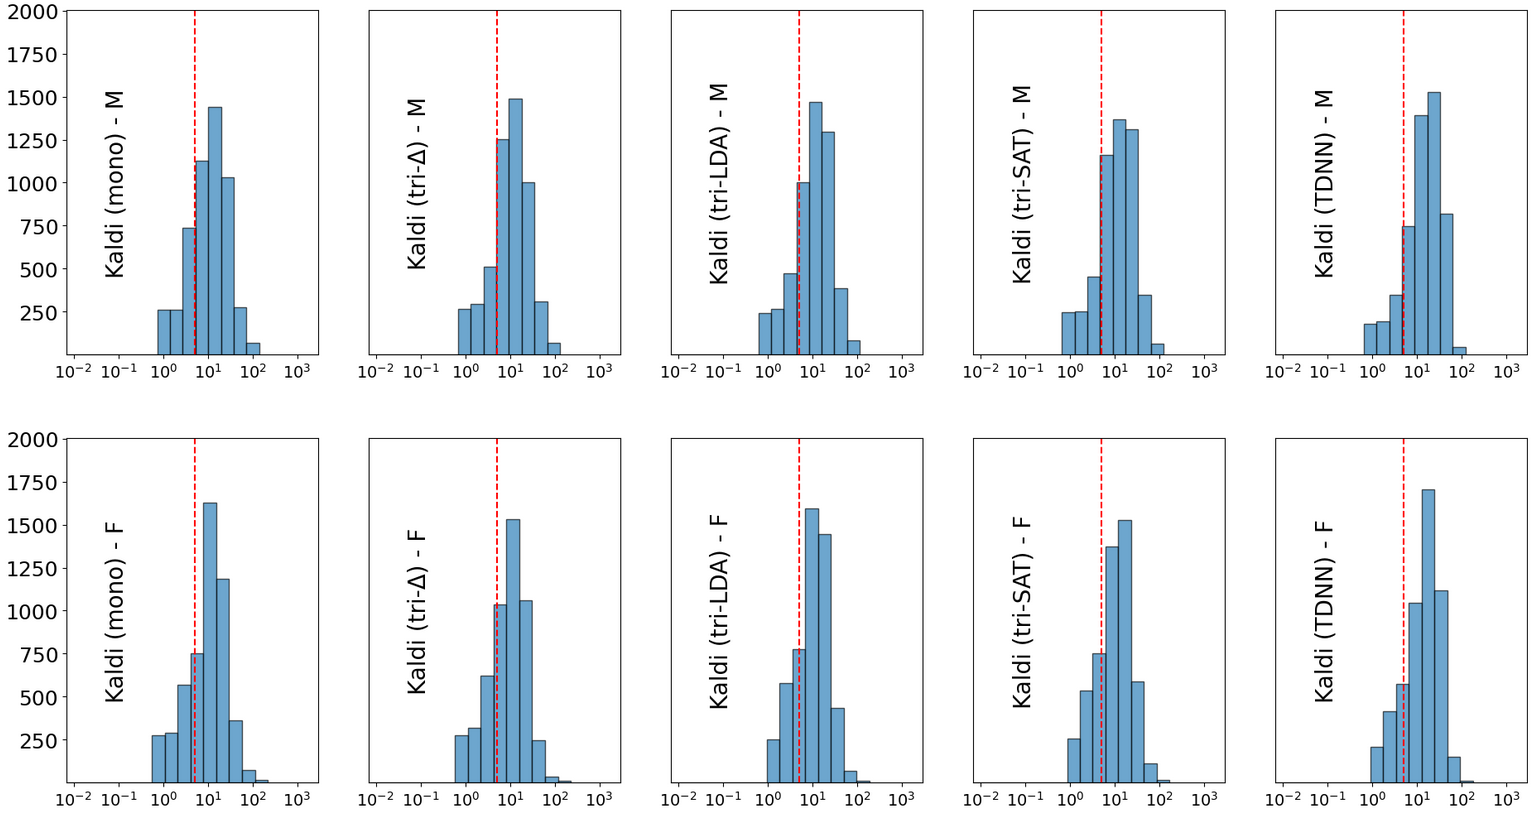
\includegraphics[width=\textwidth]{Figures/eurasip}
\end{center}
\caption{Histograma dos limites fon\'eticos entre o alinhamento for\c{c}ado e o alinhamento manual}
\end{figure}
\end{frame}

\begin{frame}
    \frametitle{Conclus�o}
    \begin{itemize}
        \item Os modelos ac�sticos treinados utilizando o Kaldi obtiveram resultados superiores � outros com suporte � l�ngua portuguesa, e t�o satisfat�rios quanto modelos para outras l�nguas
        \item Foi desenvolvido uma interface para utiliza��o do alinhador
        \item Fatores positivos:
            \begin{itemize}
                \item Avan�os na �rea de reconhecimento de voz para PT-BR
                \item Disponibiliza��o dos recursos desenvolvidos: \url{https://ufpafalabrasil.gitlab.io/}
            \end{itemize}
    \end{itemize}
\end{frame}

% \subsection{Trabalhos Futuros}
% % ----------------------------------------------------------------------------
% \begin{frame}{Trabalhos Futuros}
% \begin{itemize}
% % \item Expandir para outros sistemas operacionais: Windows, MacOS Android
% \item Solu��o alternativa ao \textit{headset}
% \item Sensores alternativos: Microfones de eletreto, BMP180 (press�o)
% \end{itemize}
% \end{frame}
%%% EOF %%%


%%%%%%%%%%%%%%%%%%%%%%%%%%%%%%%%%%%%%%%%%
%%% end of body
%%%%%%%%%%%%%%%%%%%%%%%%%%%%%%%%%%%%%%%%%

\section*{}
\renewcommand*{\currentname}{Agradecimentos}
% ------------------------------------------------------------------------------
\begin{frame}{Agradecimentos}
\begin{figure}
	\centering
	
\includegraphics[width=0.3\textwidth]{Figures/logo_ufpa}
	% 
\includegraphics[width=0.4\textwidth]{Figures/propesp} \quad
    
\includegraphics[width=0.2\textwidth]{Figures/falabrasil}
	
\includegraphics[width=0.4\textwidth]{Figures/pibic}
	% 
\includegraphics[width=0.4\textwidth]{Figures/pibex2}
\end{figure}



%\begin{center}
%\begin{figure}
%	\includegraphics[width=0.20\textwidth]{Figures/calabriano}
%	\quad\quad
%	\includegraphics[width=0.25\textwidth]{Figures/appd}\\[12pt]
%	
\includegraphics[width=0.20\textwidth]{Figures/logo_ufpa}
%	\quad\quad
%	
\includegraphics[width=0.30\textwidth]{Figures/cnpq}
%\end{figure}
%\end{center}
\end{frame}
% ------------------------------------------------------------------------------

% ------------------------------------------------------------------------------
%\begin{frame}{Agradecimentos}
%\begin{center}
%\begin{figure}
%	\includegraphics[width=0.85\textwidth]{Figures/voluntarios}
%\end{figure}
%\end{center}
%\end{frame}
% ------------------------------------------------------------------------------

\section*{}
\renewcommand*{\currentname}{Thanks}
%\setbeamertemplate{footline}
%{%
%	\begin{beamercolorbox}[wd=\paperwidth,ht=0.5ex,dp=0ex,center]{footlinerule}
%	\end{beamercolorbox}%
%	\begin{beamercolorbox}[wd=\paperwidth,ht=0.6ex,dp=0ex,center]{empty}
%	\end{beamercolorbox}%
%	\leavevmode%
%	\hbox{%
%
%	\begin{beamercolorbox}[wd=.20\paperwidth,ht=2.25ex,dp=2ex,center]{author in head/foot}%
%		\usebeamerfont{author in head/foot}%
%		%\insertshortauthor\hspace{1em}
%	\end{beamercolorbox}%
%
%	\begin{beamercolorbox}[wd=.45\paperwidth,ht=2.25ex,dp=2ex,right]{title in head/foot}%
%		\usebeamerfont{title in head/foot}
%		%\insertshorttitle
%	\end{beamercolorbox}%
%
%	\begin{beamercolorbox}[wd=.20\paperwidth,ht=2.25ex,dp=2ex,right]{author in head/foot}%
%		\usebeamerfont{author in head/foot}%
%		\textbf{\textcolor{black}{\currentname}}
%	\end{beamercolorbox}%
%
%	\begin{beamercolorbox}[wd=.10\paperwidth,ht=2.25ex,dp=2ex,right]{date in head/foot}%
%		\textbf{\textcolor{black}{\insertframenumber{} of \inserttotalframenumber\hspace*{1ex}}}
%	\end{beamercolorbox}}%
%	\vskip0pt%
%}%
% ------------------------------------------------------------------------------
\begin{frame}
\author{}
\institute{
	\fontsize{34pt}{34pt}\selectfont
	\textcolor{blue!50!black}{\bf Obrigado!}\\[12pt]
}
\date{
	\normalsize
    Jo�o Canavarro (\href{mailto:jvcanavarro@icen.ufpa.br}{\tt jvcanavarro@ufpa.br})\\[1pt]
	Universidade Federal do Par� (UFPA)\\[1pt]
	Bel�m -- Par� -- Brasil\\
}
\titlepage
\end{frame}
\end{document}
%%% EOF %%%
